% This is text associated with the open textbook "Open Electromagnetics"
% See immediately below for author, date
% This work is licensed under the Creative Commons Attribution-ShareAlike 4.0 International License. (CC BY-SA 4.0) 
% To view a copy of the license, visit http://creativecommons.org/licenses/by-sa/4.0/

%ORB TITLE Vector Arithmetic
%ORB AUTHOR 0        # S.W. Ellingson, Virginia Tech (ellingson@vt.edu)
%ORB DATE 20180803   # yyyymmdd
%ORB ABSTRACT Vector Arithmetic

\label{m0006_Vector_Arithmetic} % <-- Must match name of this file and module directory name.  Don't mess with this!
\index{vector!arithmetic|(}

A \emph{vector} 
\index{vector!definition}
is a mathematical object that has both a scalar part (i.e., a magnitude and possibly a phase), as well as a direction.
Many physical quantities are best described as vectors.
For example, the rate of movement through space can be described as \emph{speed}; i.e., as a scalar having SI base units of m/s.
However, this quantity is more completely described as \emph{velocity}; 
\index{velocity}
i.e., as a vector whose scalar part is speed and direction indicates the direction of movement.
Similarly, force 
\index{force}
is a vector whose scalar part indicates magnitude (SI base units of N), and direction indicates the direction in which the force is applied.
Electric and magnetic fields are also best described as vectors. 

In mathematical notation, a real-valued vector ${\bf A}$ is said to have a magnitude $A=\left|{\bf A}\right|$ and direction $\hat{\bf a}$ such that
%
\begin{equation}
{\bf A} = A \hat{\bf a}
\end{equation}
%
where $\hat{\bf a}$ is a unit vector 
\index{unit vector}
\index{vector!unit}
(i.e., a real-valued vector having magnitude equal to one) having the same direction as ${\bf A}$.
If a vector is complex-valued, then $A$ is similarly complex-valued.

{\bf Cartesian Coordinate System.} 
\index{Cartesian coordinate system}
Fundamentals of vector arithmetic are most easily grasped using the Cartesian coordinate system.
This system is shown in Figure~\ref{m0006_fCartesian}.
Note carefully the relative orientation of the $x$, $y$, and $z$ axes.
This orientation is important. 
For example, there are two directions that are perpendicular to the $z=0$ plane (in which the $x$- and $y$-axes lie), but the $+z$ axis is specified to be one of these in particular.  
%
\begin{figure}
\begin{center}
\pdftooltip{{  % note double brac
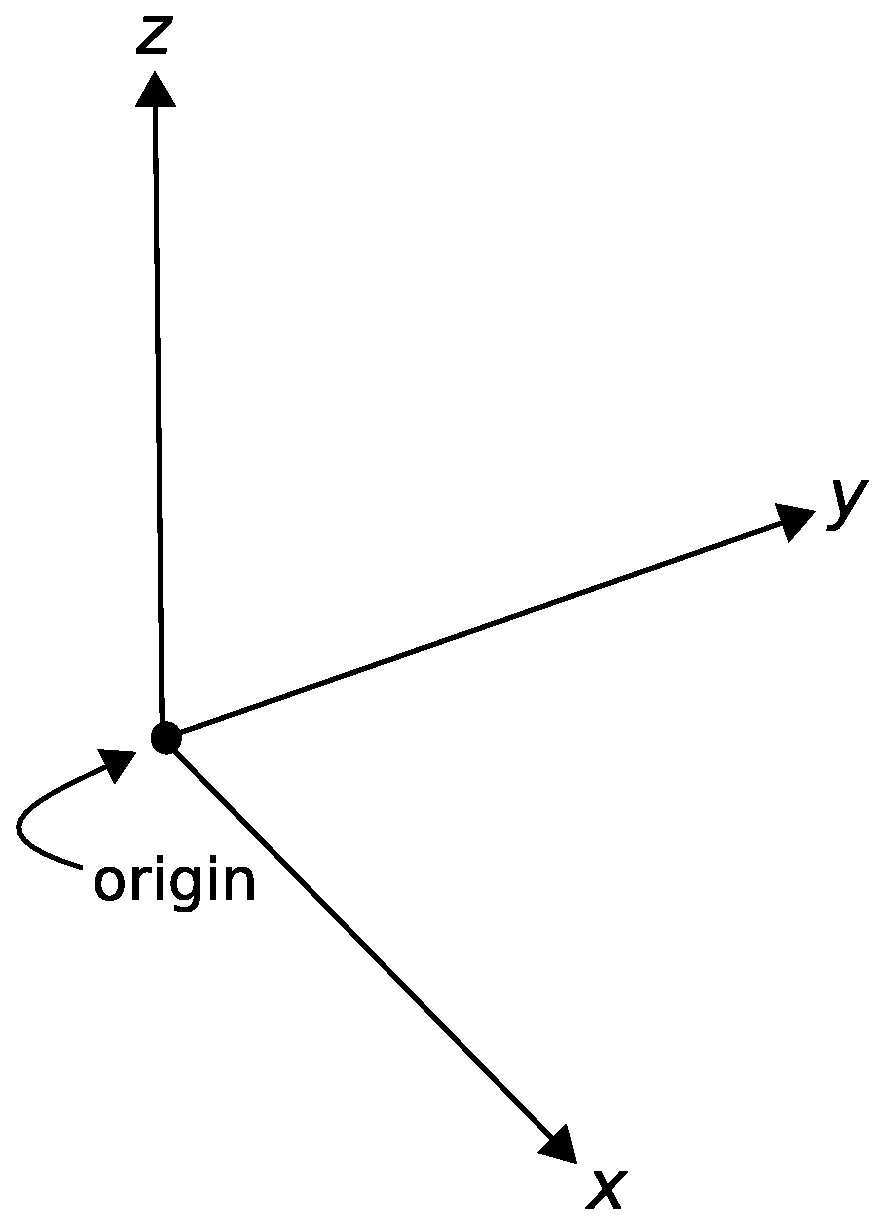
\includegraphics[width=1.5in]{modules/m0006_fCartesian.eps} 
% https://commons.wikimedia.org/wiki/File:M0006_fCartesian.svg
}}{x, y, and z axes. The z-axis points vertically. The y-axis and x-axis are perpendicular to the z-axis and to one another. They are connected at the origin.}
\end{center}
\centerline{\scriptsize 
\copyright~\hyperref[m0006_fCartesian_Credit]{K.\ Kikkeri} 
\href{https://creativecommons.org/licenses/by-sa/4.0/}{CC BY~SA 4.0} 
} 
\caption{
\label{m0006_fCartesian}
Cartesian coordinate system.
}
\end{figure}

{\bf Position-Fixed vs. Position-Free Vectors.} 
\index{vector!position-fixed}
\index{vector!position-free}
It is often convenient to describe a position in space as a vector for which the magnitude is the distance from the origin of the coordinate system and for which the direction is measured from the origin toward the position of interest.
This is shown in Figure~\ref{m0006_fPositionFixed}.
These \emph{position vectors} are ``position-fixed'' in the sense that they are defined with respect to a single point in space, which in this case is the origin.  Position vectors can also be defined as vectors that are defined with respect to some other point in space, in which case they are considered position-fixed to that position.
%
\begin{figure}
\begin{center}
\pdftooltip{{  % note double braces
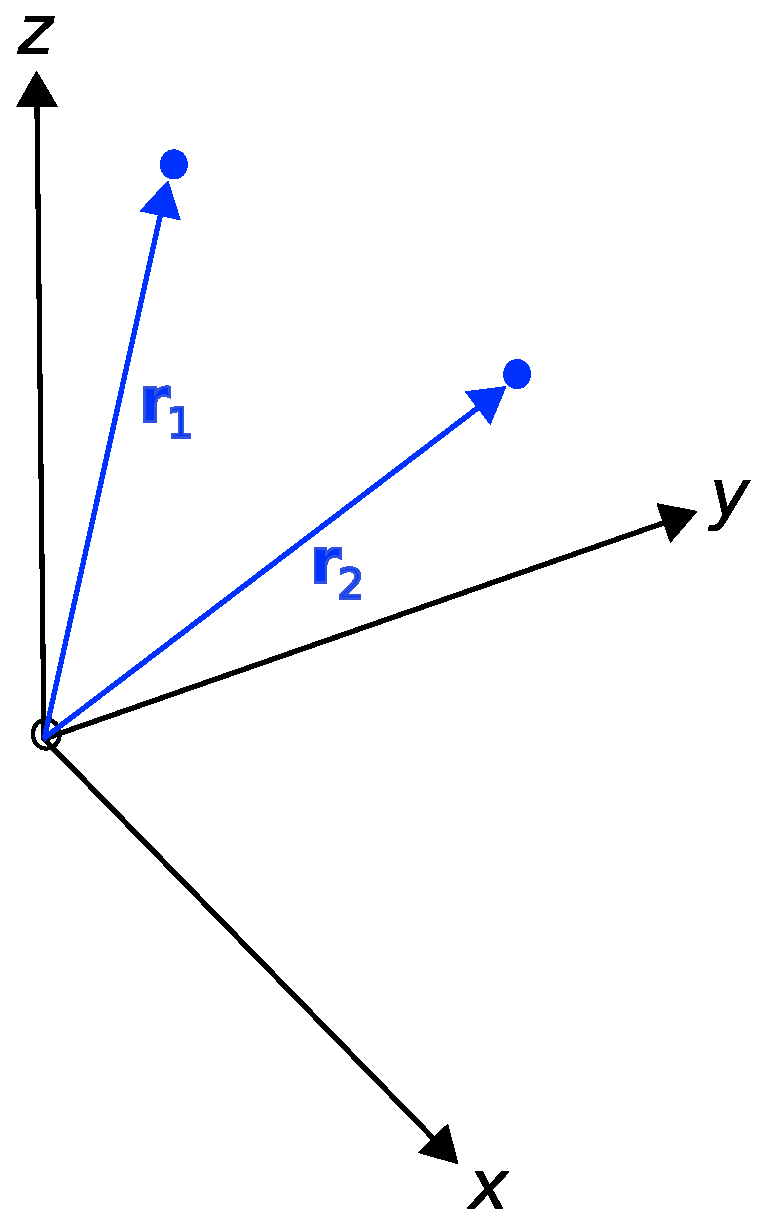
\includegraphics[width=1.5in]{modules/m0006_fPositionFixed.eps}
% https://commons.wikimedia.org/wiki/File:M0006_fPositionFixed.svg
}}{The same Cartesian coordinate system shown in a previous figure. Two blue points are arbitrarily plotted in the 3D space. There is a blue arrow pointing to each of the points from the origin. These represent vectors r sub 1 and r sub 2.}
\end{center} 
\centerline{\scriptsize 
\copyright~\hyperref[m0006_fPositionFixed_Credit]{K.\ Kikkeri} 
\href{https://creativecommons.org/licenses/by-sa/4.0/}{CC BY~SA 4.0} 
} 
\caption{
\label{m0006_fPositionFixed}
Position vectors. The vectors ${\bf r}_1$ and ${\bf r}_1$ are position-fixed and refer to particular locations.
}
\end{figure}

\emph{Position-free} vectors, on the other hand, are not defined with respect to a particular point in space.  
An example is shown in Figure~\ref{m0006_fPositionFree}.
Particles 1~m apart may both be traveling at 2~m/s in the same direction.  
In this case, the velocity of each particle can be described using the same vector, even though the particles are located at different points in space. 
%
\begin{figure}
\begin{center}
\pdftooltip{{  % note double braces
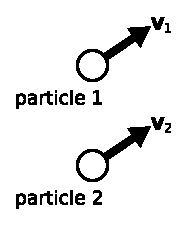
\includegraphics[width=1in]{modules/m0006_fPositionFree.eps}
% https://commons.wikimedia.org/wiki/File:M0006_fPositionFree.svg
}}{Two diagrams, one below the other. The top diagram shows an arrow of arbitrary length and direction pointing out of an empty circle. This arrow is labeled v sub 1 and the empty circle is particle 1. The bottom diagram is identical except the arrow is labeled v sub 2  and the empty circle is particle 2.}
\end{center} 
\centerline{\scriptsize 
\copyright~\hyperref[m0006_fPositionFree_Credit]{K.\ Kikkeri} 
\href{https://creativecommons.org/licenses/by-sa/4.0/}{CC BY~SA 4.0} 
} 
\caption{
\label{m0006_fPositionFree}
Two particles exhibiting the same velocity.  In this case, the velocity vectors ${\bf v}_1$ and ${\bf v}_2$ are position-free and equal.
}
\end{figure}

Position-free vectors are said to be equal if they have the same magnitudes and directions.
Position-fixed vectors, on the other hand, must also be referenced to the same position (e.g., the origin) to be considered equal.

{\bf Basis Vectors.} 
Each coordinate system is defined in terms of three basis vectors which concisely describe all possible ways to traverse three-dimensional space. 
A basis vector is a position-free unit vector that is perpendicular to all other basis vectors for that coordinate system. 
The basis vectors $\hat{\bf x}$, $\hat{\bf y}$, and $\hat{\bf z}$ of the Cartesian coordinate system are shown in Figure~\ref{m0006_fCartesianBasis}. 
In this notation, $\hat{\bf x}$ indicates the direction in which $x$ increases most rapidly, $\hat{\bf y}$ indicates the direction in which $y$ increases most rapidly, and $\hat{\bf z}$ indicates the direction in which $z$ increases most rapidly.
Alternatively, you might interpret $\hat{\bf x}$, $\hat{\bf y}$, and $\hat{\bf z}$ as unit vectors that are parallel to the $x$-, $y$-, and $z$-axes and point in the direction in which values along each axis increase.
%
\begin{figure}
\begin{center}
\pdftooltip{{  % note double braces
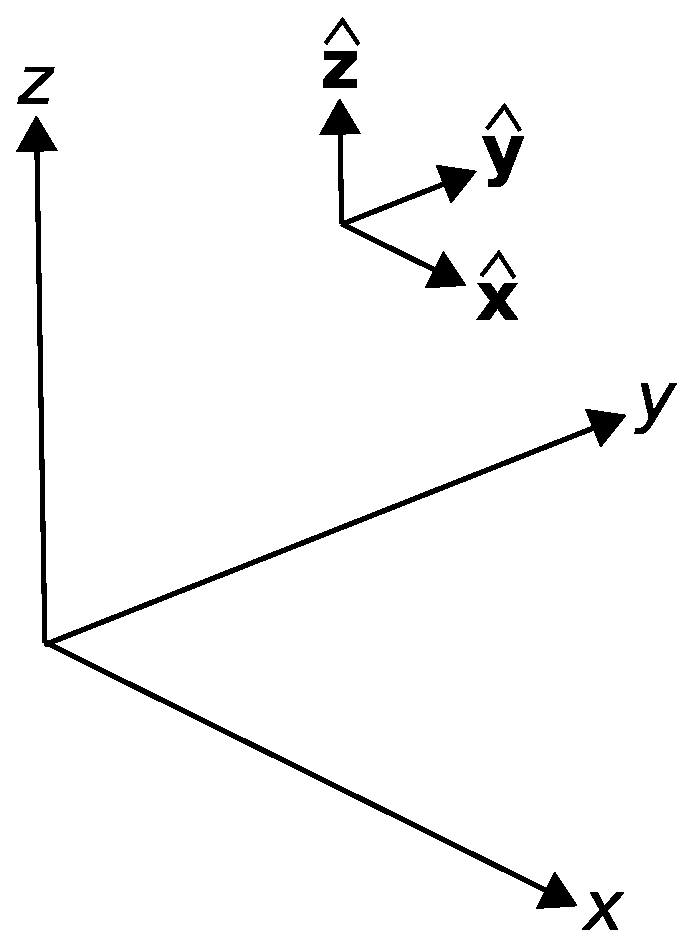
\includegraphics[width=1.5in]{modules/m0006_fCartesianBasis.eps}
% https://commons.wikimedia.org/wiki/File:M0006_fCartesianBasis.svg
}}{Shows the same Cartesian coordinate system from a previous figure. Overlayed on this is a smaller version of the coordinate system with the axes labeled x-hat, y-hat, and z-hat to correspond with the axis labels of the larger coordinate system.}
\end{center} 
\centerline{\scriptsize 
\copyright~\hyperref[m0006_fCartesianBasis_Credit]{K.\ Kikkeri} 
\href{https://creativecommons.org/licenses/by-sa/4.0/}{CC BY~SA 4.0} 
} 
\caption{
\label{m0006_fCartesianBasis}
Basis vectors in the Cartesian coordinate system.
}
\end{figure}

{\bf Vectors in the Cartesian Coordinate System.}
In Cartesian coordinates, we may describe any vector ${\bf A}$ as follows:
%
\begin{equation}
{\bf A} = \hat{\bf x}A_x + \hat{\bf y}A_y + \hat{\bf z}A_z
\end{equation} 
%
where $A_x$, $A_y$, and $A_z$ are scalar quantities describing the components of ${\bf A}$ in each of the associated directions, as shown in Figure~\ref{m0006_fVecCart}.
This description makes it clear that the magnitude of ${\bf A}$ is:
%
\begin{equation}
\left|{\bf A}\right| = \sqrt{ A_x^2 + A_y^2 + A_z^2 }
\end{equation}
%
and therefore, we can calculate the associated unit vector as
%
\begin{equation}
\begin{split}
\hat{\bf a} &= \frac{\bf A}{\left|{\bf A}\right|} = \frac{\bf A}{\sqrt{ A_x^2 + A_y^2 + A_z^2 }} \\
            &= ~~~\hat{\bf x}A_x \left( A_x^2 + A_y^2 + A_z^2 \right)^{-1/2} \\
            &~ ~~+\hat{\bf y}A_y \left( A_x^2 + A_y^2 + A_z^2 \right)^{-1/2} \\
            &~ ~~+\hat{\bf z}A_z \left( A_x^2 + A_y^2 + A_z^2 \right)^{-1/2} 
\end{split}
\end{equation}
%
\begin{figure}
\begin{center}
\pdftooltip{{  % note double braces
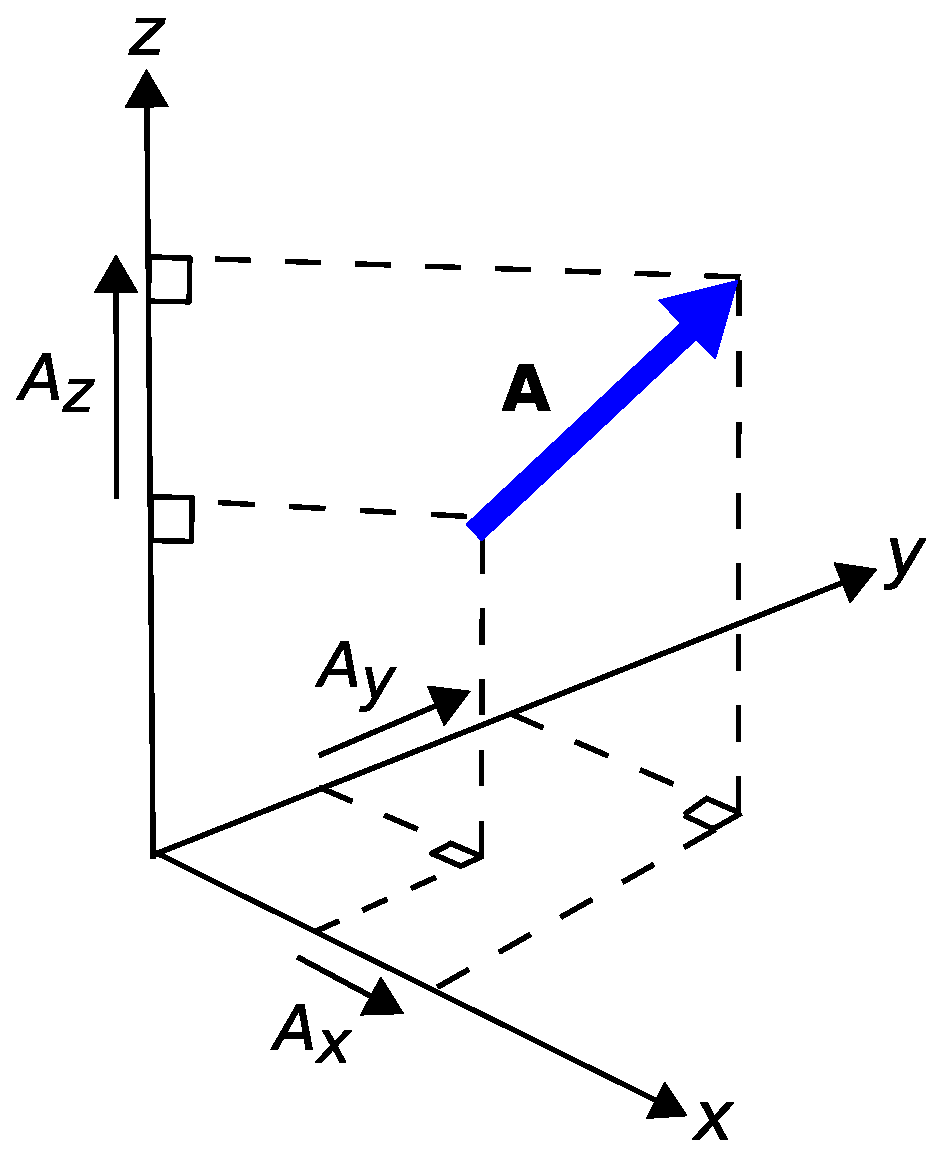
\includegraphics[width=2in]{modules/m0006_fVecCart.eps}
% https://commons.wikimedia.org/wiki/File:M0006_fVecCart.svg
}}{An arrow with a positive slope is arbitrarily positioned on the three dimensional Cartesian coordinate system. Dashed lines map the head and tail of the vector to each plane. The distances between the tale and head projection points on each axis are labeled A sub x, A sub y, and A sub z representing vector components.}
\end{center} 
\centerline{\scriptsize 
\copyright~\hyperref[m0006_fVecCart_Credit]{K.\ Kikkeri} 
\href{https://creativecommons.org/licenses/by-sa/4.0/}{CC BY~SA 4.0} 
} 
\caption{
\label{m0006_fVecCart}
Components of a vector ${\bf A}$ in the Cartesian coordinate system.
}
\end{figure}

{\bf Vector Addition and Subtraction.}
It is common to add and subtract vectors.
For example, vectors describing two forces ${\bf A}$ and ${\bf B}$ applied to the same point can be described as a single force vector ${\bf C}$ that is the sum of ${\bf A}$ and ${\bf B}$; i.e., ${\bf C}={\bf A}+{\bf B}$.
This addition is quite simple in the Cartesian coordinate system:
%
\begin{equation}
\begin{split}
{\bf C} &= {\bf A}+{\bf B} \\
        &= \left(\hat{\bf x}A_x + \hat{\bf y}A_y + \hat{\bf z}A_z\right) + \left( \hat{\bf x}B_x + \hat{\bf y}B_y + \hat{\bf z}B_z \right) \\
        &= \hat{\bf x}\left(A_x+B_x\right) + \hat{\bf y}\left(A_y+B_y\right) + \hat{\bf z}\left(A_z+B_z\right) 
\end{split}
\end{equation}
%
In other words, the $\hat{\bf x}$ component of ${\bf C}$ is the sum of the $\hat{\bf x}$ components of ${\bf A}$ and ${\bf B}$, and similarly for $\hat{\bf y}$ and $\hat{\bf z}$.
From the above example, it is clear that vector addition is commutative; i.e., 
%
\begin{equation}
{\bf A}+{\bf B} = {\bf B}+{\bf A}
\end{equation}
%
In other words, vectors may be added in any order.
Vector subtraction is defined similarly:
%
\begin{equation}
\begin{split}
{\bf D} &= {\bf A}-{\bf B} \\
        &= \left(\hat{\bf x}A_x + \hat{\bf y}A_y + \hat{\bf z}A_z\right) - \left( \hat{\bf x}B_x + \hat{\bf y}B_y + \hat{\bf z}B_z \right) \\
        &= \hat{\bf x}\left(A_x-B_x\right) + \hat{\bf y}\left(A_y-B_y\right) + \hat{\bf z}\left(A_z-B_z\right) 
\end{split}
\end{equation}
%
In other words, the $\hat{\bf x}$ component of ${\bf D}$ is the difference of the $\hat{\bf x}$ components of ${\bf A}$ and ${\bf B}$, and similarly for $\hat{\bf y}$ and $\hat{\bf z}$.
Like scalar subtraction, vector subtraction is \emph{not} commutative.

{\bf Relative Positions and Distances.}
A common task in vector analysis is to describe the position of one point in space relative to a different point in space. 
 Let us identify those two points using the position vectors ${\bf r}_1$ and ${\bf r}_2$, as indicated in Figure~\ref{m0006_fRelativePosition}. We may identify a third vector ${\bf r}_{12}$ as the position of ${\bf r}_{2}$ relative to ${\bf r}_{1}$:
%
\begin{equation}
{\bf r}_{12} \triangleq {\bf r}_{2} - {\bf r}_{1}
\end{equation}
%
Now $\left|{\bf r}_{12}\right|$ is the distance between these points, and ${\bf r}_{12}/\left|{\bf r}_{12}\right|$ is a unit vector indicating the direction to ${\bf r}_{2}$ from ${\bf r}_{1}$. 
%
\begin{figure}
\begin{center}
\pdftooltip{{  % note double brace
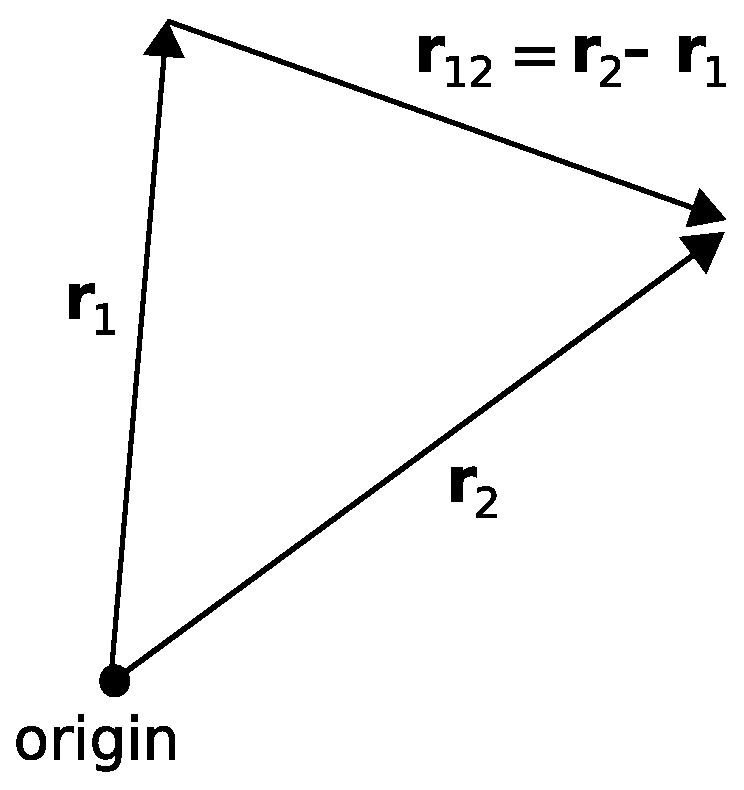
\includegraphics[width=1.5in]{modules/m0006_fRelativePosition.eps}
% https://commons.wikimedia.org/wiki/File:M0006_fRelativePosition.svg
}}{Two vectors of arbitrary lengths and direction, r sub 1 and r sub 2, emanate from the same point of origin. A third vector, r sub 12, starts at the head of r sub 1 and ends at the head of r sub 2. The third vector is labeled r sub 12 = r sub 2 - r sub 1.}
\end{center} 
\centerline{\scriptsize 
\copyright~\hyperref[m0006_fRelativePosition_Credit]{K.\ Kikkeri} 
\href{https://creativecommons.org/licenses/by-sa/4.0/}{CC BY~SA 4.0} 
} 
\caption{
\label{m0006_fRelativePosition}
Relative position (distance and direction) between locations identified by their position vectors.
}
\end{figure}

%%%%%%%%%%%%%%%%%%%%%%%%%%%%%%%%%%%%%%%%%%%%%%%%%%%%%%

%ORB EXAMPLE
~\\ \begin{example} 
\begin{mdframed}[backgroundcolor=brown!20,linecolor=brown!20]\raggedright
Direction and distance between positions.
\\~\\
Consider two positions, identified using the position vectors
${\bf r}_1 = 2\hat{\bf x} +3\hat{\bf y} +1\hat{\bf z}$ and
${\bf r}_2 = 1\hat{\bf x} -2\hat{\bf y} +3\hat{\bf z}$, both expressed in units of meters.
Find the direction vector that points from ${\bf r}_1$ to ${\bf r}_2$, the distance between these points, and the associated unit vector.

{\bf Solution.}
The vector that points from ${\bf r}_1$ to ${\bf r}_2$ is 
%
\begin{flalign}
{\bf R}  &= {\bf r}_2 - {\bf r}_1 \nonumber \\
         &= (1-2)\hat{\bf x} +(-2-3)\hat{\bf y} +(3-1)\hat{\bf z} \nonumber \\
         &= -\hat{\bf x} -5\hat{\bf y} +2\hat{\bf z} 
\end{flalign}
%
The distance between ${\bf r}_1$ and ${\bf r}_2$ is simply the magnitude of this vector:
%
\begin{equation}
\left|{\bf R}\right| = \sqrt{ \left(-1\right)^2  + \left(-5\right)^2  + \left(2\right)^2 } \cong 5.48~\mbox{m}
\end{equation}
%
The unit vector $\hat{\bf R}$ is simply ${\bf R}$ normalized to have unit magnitude:
%
\begin{flalign}
\hat{\bf R} &= {\bf R}/\left|{\bf R}\right| \nonumber \\
            &\cong \left(-\hat{\bf x} -5\hat{\bf y} +2\hat{\bf z}\right)/5.48 \nonumber \\
            &\cong -0.182\hat{\bf x} -0.913\hat{\bf y} +0.365\hat{\bf z}  
\end{flalign}

\end{mdframed}\end{example}


%---------------------------------------------------------------------------

{\bf Multiplication of a Vector by a Scalar.}
Let's say a particular force is specified by a vector ${\bf F}$.  What is the new vector if this force is doubled?  The answer is simply $2{\bf F}$ -- that is, twice the magnitude applied in the same direction.  This is an example of scalar multiplication of a vector.  Generalizing, the product of the scalar $\alpha$ and the vector ${\bf A}$ is simply $\alpha{\bf A}$.

\index{dot product|(}
\index{scalar product|see{dot product}}
{\bf Scalar (``Dot'') Product of Vectors.}
Another common task in vector analysis is to determine the similarity in the direction in which two vectors point.
In particular, it is useful to have a metric which, when applied to the vectors ${\bf A}=\hat{\bf a}A$ and ${\bf B}=\hat{\bf b}B$, has the following properties (see Figure~\ref{m0006_fDotProductSpecialCases}):
%
\begin{itemize}
\item If ${\bf A}$ is perpendicular to ${\bf B}$, the result is zero.
\item If ${\bf A}$ and ${\bf B}$ point in the same direction, the result is $AB$.
\item If ${\bf A}$ and ${\bf B}$ point in opposite directions, the result is $-AB$.
\item Results intermediate to these conditions depend on the angle $\psi$ between ${\bf A}$ and ${\bf B}$, measured as if ${\bf A}$ and ${\bf B}$ were arranged ``tail-to-tail'' as shown in Figure~\ref{m0006_fDotProduct}.
\end{itemize}
%
\begin{figure}
\begin{center}
\pdftooltip{{  % note double braces
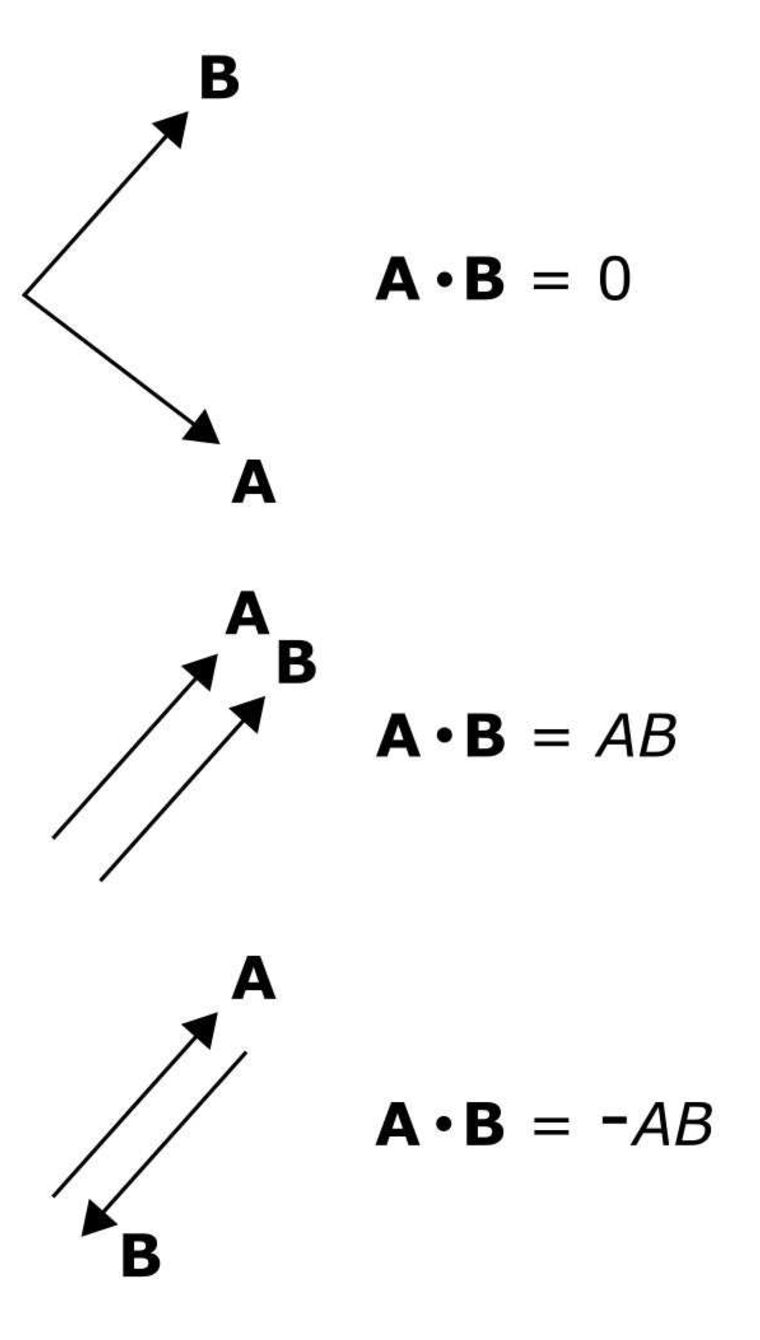
\includegraphics[width=1.5in]{modules/m0006_fDotProductSpecialCases.eps}
% https://commons.wikimedia.org/wiki/File:M0006_fDotProductSpecialCases.svg
}}{Three diagrams: top, middle, and bottom.
Top: Vectors A and B are perpendicular. vector A dot vector B = 0
Middle: Vectors A and B are parallel in the same direction. vector A dot vector B = AB
Bottom: Vectors A and B are parallel in opposite directions. vector A dot vector B = -AB
}
\end{center} 
\centerline{\scriptsize 
\copyright~\hyperref[m0006_fDotProductSpecialCases_Credit]{K.\ Kikkeri} 
\href{https://creativecommons.org/licenses/by-sa/4.0/}{CC BY~SA 4.0} 
} 
\caption{
\label{m0006_fDotProductSpecialCases}
Special cases of the dot product.
}
\end{figure}
%
In vector analysis, this operator is known as the \emph{scalar product} (not to be confused with scalar multiplication) or the \emph{dot product}.  
The dot product is written ${\bf A}\cdot{\bf B}$
and is given in general by the expression:
%
\begin{equation}
{\bf A}\cdot{\bf B} = AB\cos\psi
\label{m0006_eDPdef}
\end{equation}
%
Note that this expression yields the special cases previously identified, which are $\psi=\pi/2$, $\psi=0$, and $\psi=\pi$, respectively.
The dot product is commutative; i.e., 
%
\begin{equation}
{\bf A}\cdot{\bf B} = {\bf B}\cdot{\bf A} 
\end{equation}
%
The dot product is also distributive; i.e., 
%
\begin{equation}
{\bf A}\cdot\left({\bf B}+{\bf C}\right) = {\bf A}\cdot{\bf B}+{\bf A}\cdot{\bf C}
\end{equation}
%
\begin{figure}
\begin{center}
\pdftooltip{{  % note double braces
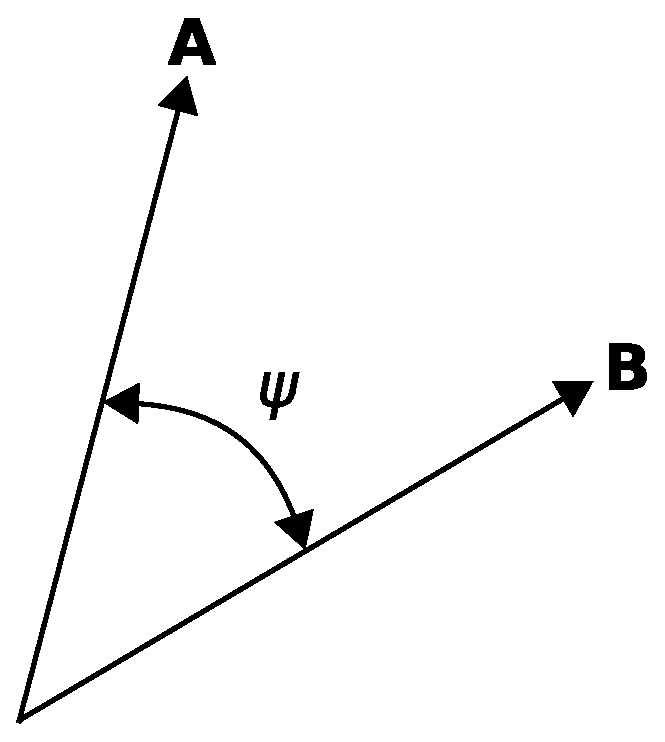
\includegraphics[width=1.5in]{modules/m0006_fDotProduct.eps}
% https://commons.wikimedia.org/wiki/File:M0006_fDotProduct.svg
}}{Vectors A and B emanate from the same point of origin to form an arbitrary acute angle. The angle between them is labeled psi.}
\end{center} 
\centerline{\scriptsize 
\copyright~\hyperref[m0006_fDotProduct_Credit]{K.\ Kikkeri} 
\href{https://creativecommons.org/licenses/by-sa/4.0/}{CC BY~SA 4.0} 
} 
\caption{
\label{m0006_fDotProduct}
Calculation of the dot product.
}
\end{figure}

The dot product has some other useful properties.
For example, note:
%
\begin{equation}
\begin{split}
{\bf A}\cdot{\bf A} &= \left(\hat{\bf x}A_x + \hat{\bf y}A_y + \hat{\bf z}A_z\right) \cdot \left(\hat{\bf x}A_x + \hat{\bf y}A_y + \hat{\bf z}A_z\right) \\
                    &= ~~\hat{\bf x}\cdot\hat{\bf x} A_x^2 + \hat{\bf x}\cdot\hat{\bf y} A_x A_y + \hat{\bf x}\cdot\hat{\bf z} A_x A_z \\
                    &~~  +\hat{\bf y}\cdot\hat{\bf x} A_x A_y + \hat{\bf y}\cdot\hat{\bf y} A_y^2 + \hat{\bf y}\cdot\hat{\bf z} A_y A_z \\
                    &~~  +\hat{\bf z}\cdot\hat{\bf x} A_x A_z + \hat{\bf z}\cdot\hat{\bf y} A_y A_z + \hat{\bf z}\cdot\hat{\bf z} A_z^2 
\end{split}
\end{equation}
%
which looks pretty bad until you realize that 
%
\begin{equation}
\hat{\bf x}\cdot\hat{\bf x} = \hat{\bf y}\cdot\hat{\bf y} = \hat{\bf z}\cdot\hat{\bf z} = 1
\end{equation}
%
and any other dot product of basis vectors is zero.  Thus, the whole mess simplifies to:
%
\begin{equation}
{\bf A}\cdot{\bf A} = A_x^2 + A_y^2 + A_z^2
\end{equation}
%
This is the square of the magnitude of ${\bf A}$, so we have discovered that
%
\begin{equation}
{\bf A}\cdot{\bf A} = \left|{\bf A}\right|^2 = A^2
\end{equation}
%
Applying the same principles to the dot product of potentially different vectors ${\bf A}$ and ${\bf B}$, we find:
%
\begin{equation}
\begin{split}
{\bf A}\cdot{\bf B} &= \left(\hat{\bf x}A_x + \hat{\bf y}A_y + \hat{\bf z}A_z\right) \cdot \left(\hat{\bf x}B_x + \hat{\bf y}B_y + \hat{\bf z}B_z\right) \\
                    &= A_x B_x + A_y B_y + A_z B_z
\end{split}
\label{m0006_eDPC}
\end{equation}
%
This is a particularly easy way to calculate the dot product, since it eliminates the problem of determining the angle $\psi$.
In fact, an easy way to calculate $\psi$ given ${\bf A}$ and ${\bf B}$ is to first calculate the dot product using Equation~\ref{m0006_eDPC} and then use the result to solve Equation~\ref{m0006_eDPdef} for $\psi$.

%ORB EXAMPLE
~\\ \begin{example} 
\begin{mdframed}[backgroundcolor=brown!20,linecolor=brown!20]\raggedright
Angle between two vectors. 
\\~\\
Consider the position vectors
${\bf C} = 2\hat{\bf x} +3\hat{\bf y} +1\hat{\bf z}$ and
${\bf D} = 3\hat{\bf x} -2\hat{\bf y} +2\hat{\bf z}$, both expressed in units of meters.
Find the angle between these vectors.

{\bf Solution.}
From Equation~\ref{m0006_eDPdef}
%
\begin{equation}
{\bf C}\cdot{\bf D} = CD\cos\psi
\end{equation}
%
where $C = \left|{\bf C}\right|$, $D = \left|{\bf D}\right|$, and $\psi$ is the angle we seek.
From Equation~\ref{m0006_eDPC}:
%
\begin{flalign}
{\bf C}\cdot{\bf D} &= C_x D_x + C_y D_y + C_z D_z \\
                    &= 2\cdot 3 + 3\cdot\left(-2\right) + 1\cdot 2 ~\mbox{m}^2 \\
                    &= 2 ~\mbox{m}^2
\end{flalign}
%
also
%
\begin{flalign}
C &= \sqrt{C_x^2 + C_y^2 + C_z^2} \cong 3.742~\mbox{m}  \\
D &= \sqrt{D_x^2 + D_y^2 + D_z^2} \cong 4.123~\mbox{m} 
\end{flalign}
so
%
\begin{equation}
\cos\psi = \frac{{\bf C}\cdot{\bf D}}{CD} \cong 0.130
\end{equation}
%
Taking the inverse cosine, we find $\psi=82.6^{\circ}$.

\end{mdframed}\end{example}
\index{dot product|)}

%-------------------------------------------------------------------------

\index{cross product|(}
{\bf Cross Product.}
The cross product is a form of vector multiplication that results in a vector that is perpendicular to both of the operands.
The definition is as follows:
%
\begin{equation}
{\bf A}\times{\bf B} = \hat{\bf n}AB\sin\psi_{AB}
\label{m0006_eCrossProduct}
\end{equation}
%
As shown in Figure~\ref{m0006_fCrossProduct}, the unit vector $\hat{\bf n}$ is determined by the ``right hand rule.'' 
\index{right-hand rule!cross product}
Using your right hand, curl your fingers to traverse the angle $\psi_{AB}$ beginning at ${\bf A}$ and ending at ${\bf B}$, and then $\hat{\bf n}$ points in the direction of your fully-extended thumb.  

It should be apparent that the cross product is not commutative but rather is \emph{anticommutative}; that is,
%
\begin{equation}
{\bf A}\times{\bf B} = -{\bf B}\times{\bf A} 
\end{equation}
%
You can confirm this for yourself using either Equation~\ref{m0006_eCrossProduct} or by applying the right-hand rule.

The cross product is distributive:
%
\begin{equation}
{\bf A}\times\left({\bf B} + {\bf C}\right) = {\bf A}\times{\bf B} + {\bf A}\times{\bf C} 
\end{equation}
%
\begin{figure}
\begin{center}
\pdftooltip{{  % note double braces
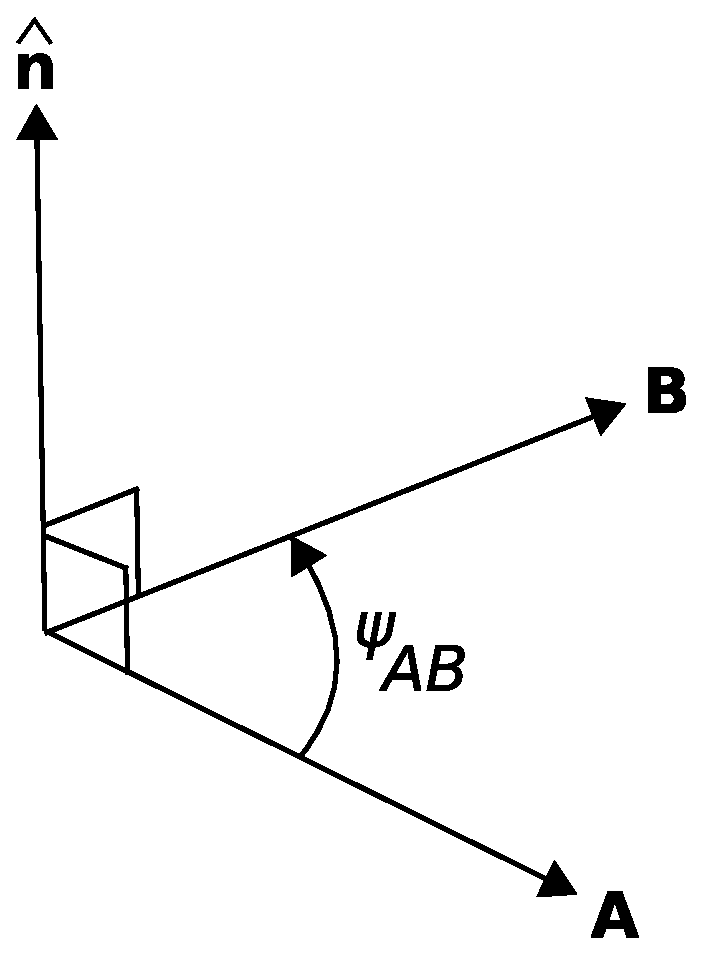
\includegraphics[width=1.5in]{modules/m0006_fCrossProduct.eps}
% https://commons.wikimedia.org/wiki/File:M0006_fCrossProduct.svg
}}{Three vectors are perpendicular to each other, labeled A, B, and n-hat. The angle formed by A and B is labeled psi sub AB}
\end{center} 
\centerline{\scriptsize 
\copyright~\hyperref[m0006_fCrossProduct_Credit]{K.\ Kikkeri} 
\href{https://creativecommons.org/licenses/by-sa/4.0/}{CC BY~SA 4.0} 
} 
\caption{
\label{m0006_fCrossProduct}
The cross product ${\bf A}\times{\bf B}$.
}
\end{figure}

There are two useful special cases of the cross product that are worth memorizing.  The first is the cross product of a vector with itself, which is zero:
%
\begin{equation}
{\bf A}\times{\bf A} = 0 
\end{equation}
%
The second is the cross product of vectors that are perpendicular; i.e., for which $\psi_{AB}=\pi/2$.  In this case:
%
\begin{equation}
{\bf A}\times{\bf B} = \hat{\bf n}AB 
\end{equation}
%
Using these principles, note:
%
\begin{equation}
\hat{\bf x} \times \hat{\bf x} = \hat{\bf y} \times \hat{\bf y} = \hat{\bf z} \times \hat{\bf z} = 0
\end{equation}
%
whereas
%
\begin{equation}
\hat{\bf x} \times \hat{\bf y} = \hat{\bf z}
\end{equation}
%
\begin{equation}
\hat{\bf y} \times \hat{\bf z} = \hat{\bf x}
\end{equation}
%
\begin{equation}
\hat{\bf z} \times \hat{\bf x} = \hat{\bf y}
\end{equation}
%
A useful diagram that summarizes these relationships is shown in Figure~\ref{m0006_fCartesianBasisCrossProducts}.
%
\begin{figure}
\begin{center}
\pdftooltip{{  % note double braces
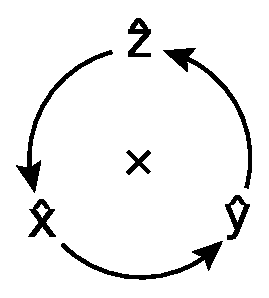
\includegraphics[width=1in]{modules/m0006_fCartesianBasisCrossProducts.eps}
}}{Arranged in a circle, x-hat, y-hat, and z-hat are arranged at 220, 300 and 90 degrees respectively. They are joined by semi-circular arrows pointing in the counter-clockwise direction. An x (cross) is at the center of the circle.}
\end{center} 
\caption{\label{m0006_fCartesianBasisCrossProducts}Cross products among basis vectors in the Cartesian system.  The cross product of any two basis vectors is the third basis vector when the order of operands is counter-clockwise, as shown in the diagram, and is $-1$ times the third basis vector when the order of operands is clockwise with respect to the arrangement in the diagram.}
\end{figure}

It is typically awkward to ``manually'' determine $\hat{\bf n}$ in Equation~\ref{m0006_eCrossProduct}.  
However, in Cartesian coordinates the cross product may be calculated as:
%
\begin{equation}
\begin{split}
{\bf A}\times{\bf B} =& ~~~~\hat{\bf x}\left(A_y B_z - A_z B_y \right) \\
                      & +\hat{\bf y}\left(A_z B_x - A_x B_z \right) \\
                      & +\hat{\bf z}\left(A_x B_y - A_y B_x \right) 
\end{split}
\end{equation}
%
This may be easier to remember as a matrix determinant:
%
\begin{equation}
{\bf A}\times{\bf B} =
\begin{vmatrix}
\hat{\bf x} & \hat{\bf y} & \hat{\bf z} \\
A_x & A_y & A_z \\
B_x & B_y & B_z 
\end{vmatrix}
\end{equation}
%
Similar expressions are available for other coordinate systems.

\index{cross product|)}

Vector analysis routinely requires expressions involving both dot products and cross products in different combinations.  Often, these expressions may be simplified, or otherwise made more convenient, using the vector identities listed in Appendix~\ref{m0140_Vector_Identities}.

%%%%%%%%%%%%%%%%%%%%%%%%%%%%%%%%%%%%

{\bf Additional Reading:}
\begin{itemize}
\item ``\href{https://en.wikipedia.org/wiki/Vector_field}{Vector field}'' on Wikipedia.
\item ``\href{https://en.wikipedia.org/wiki/Vector_algebra}{Vector algebra}'' on Wikipedia.
\end{itemize}

\index{vector!arithmetic|)}
